
\subsection*{Spielidee}
Das zweite Spiel, das von uns umgesetzt wurde, ist ein Flaggenspiel. Hierbei handelt es sich um eine Abwandlung von Capture the Flag. Es wird mit Stealth-Elementen erweitert und die Spielmechanik des Ausschaltens von Gegnern ist anders gel�st. Dieses Spiel sollte nach M�glichkeit in einer Stadt gespielt werden, da es wichtig ist in einer Menge von Passanten m�glichst unerkannt zu bleiben. Es gibt zwei Teams, die jeweils eine Basis haben. Basen werden jeweils von dem Mitglied eines Teams erstellt, welches als erstes die Erstellung �ber einen Button ausl�st. Hierbei wird als Zentrum der Basis die aktuelle Position des entsprechenden Spielers genommen. Beim betreten des Spiels, k�nnen sich Spieler zwischen Team Blau und Team Rot entscheiden. Die eigene Flagge erscheint in der N�he der eigenen Basis. Die Position der eigenen Flagge ist den Teammitgliedern unbekannt, man sieht nur die Position der gegnerischen Flagge. Die Flaggen sollen nur auf Stra�en bzw. Gehwegen (nicht in Geb�uden) zuf�llig platziert werden. Diese Platzierung wird vom Server �ber Bilderkennung bestimmt. So wird die Erreichbarkeit der Flaggen sichergestellt. Als Spieler sieht man nur die Positionen der eigenen Teammitglieder. Zur Organisation kann der Chat verwendet werden. Es ist m�glich die n�here Umgebung nach Gegnern zu scannen. Die gescannten Gegner sind dann f�r kurze zeit sichtbar. Dieses Scan-Verfahren ist jedoch nicht dauerhaft verf�gbar, sondern erst wieder m�glich nach l�ngerer Abklingzeit. Es ist m�glich potentielle Gegner zu markieren. Die Reichweite beim Markieren ist begrenzt und Richtungsabh�ngig. Hierbei wird das Smartphone auf den potentiellen Feind ausgerichtet und ein Mark-Button gedr�ckt (Auch hier besteht eine gewisse Abklingzeit). Ist dieser ein gegnerischer Mitspieler wird er markiert und ist f�r l�ngere Zeit auf der Karte sichtbar. Der Betroffene bekommt �ber seine Markierung keine R�ckmeldung. Ein Spieler, der sich in der N�he der gegnerischen Flagge befindet, kann diese aufnehmen. Um einen Spiel-Punkt zu erreichen muss die aufgenommene Flagge zur eigenen Basis gebracht werden. Dem Gegnerteam wird die Position angezeigt, an der die Flagge aufgenommen wurde. Wird ein Flaggentr�ger markiert, verliert er die Flagge und sie erscheint an einer neuen zuf�lligen Position. War der Flaggentr�ger vor der Aufnahme markiert, so ist er mit Flagge zu sehen. Wenn ein Spieler eine bestimmte Geschwindigkeit �berschreitet, wird er ebenfalls f�r das Gegnerteam sichtbar. Somit haben schnellere L�ufer keinen direkten Vorteil.
\begin{figure}
	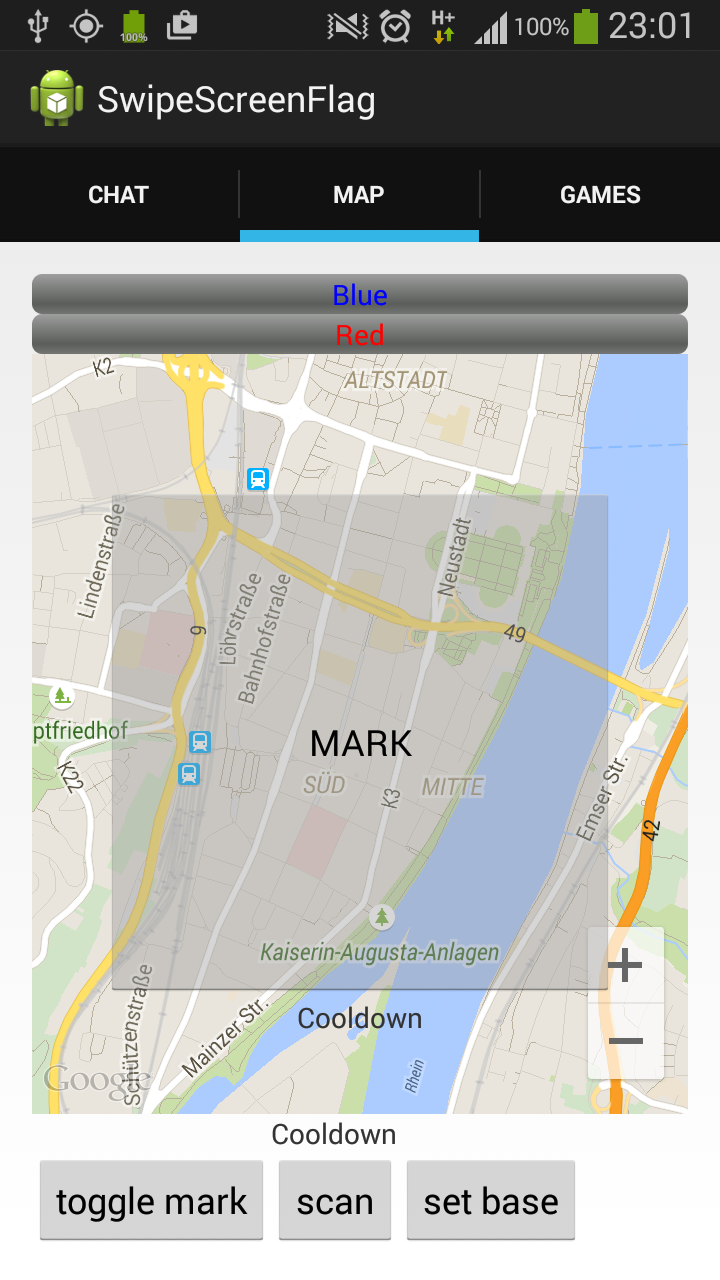
\includegraphics[width=0.5\textwidth]{5-Implementation_von_Beispielapps/5-2-Verstecken/Data/map_screen_mark_on.png}
	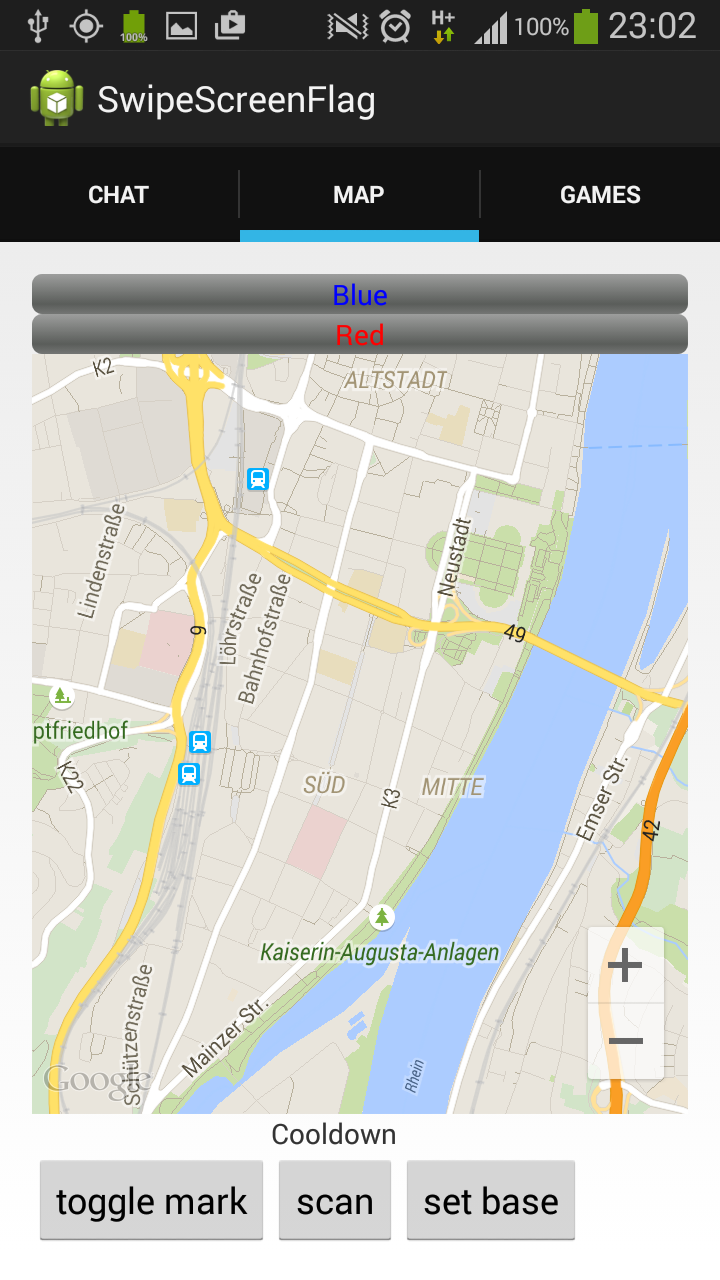
\includegraphics[width=0.5\textwidth]{5-Implementation_von_Beispielapps/5-2-Verstecken/Data/map_screen_mark_off.png}
	\caption{Map-Screen mit Mark-Button (rechts) Map-Screen ohne Mark-Button (Links)}
	\label{fig:flaggmap}
\end{figure}

